% This file was created with tikzplotlib v0.10.1.
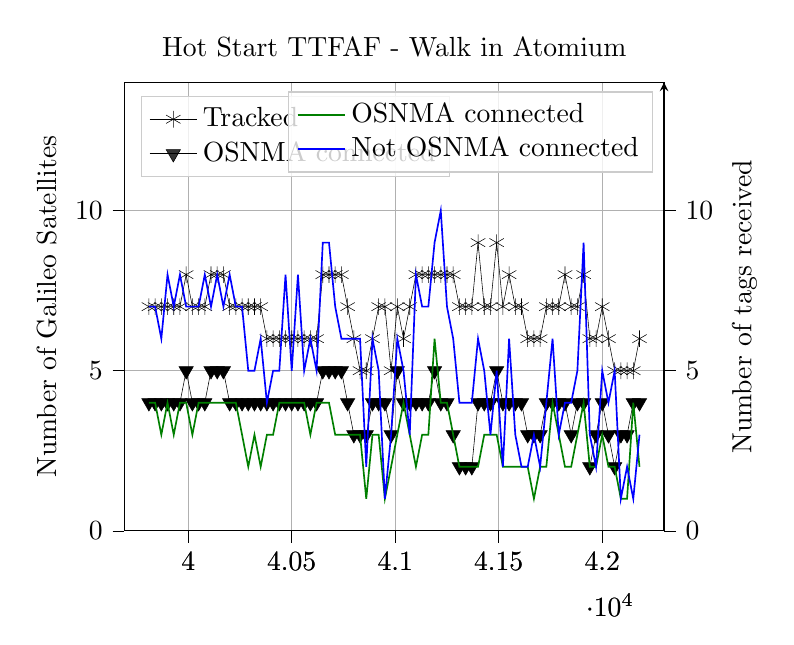
\begin{tikzpicture}

\definecolor{darkgray176}{RGB}{176,176,176}
\definecolor{green01270}{RGB}{0,127,0}
\definecolor{lightgray204}{RGB}{204,204,204}

\begin{axis}[
legend cell align={left},
legend style={
  fill opacity=0.8,
  draw opacity=1,
  text opacity=1,
  at={(0.03,0.97)},
  anchor=north west,
  draw=lightgray204
},
tick align=outside,
tick pos=left,
title={Hot Start TTFAF - Walk in Atomium},
x grid style={darkgray176},
xmajorgrids,
xmin=39691.5, xmax=42298.5,
xtick style={color=black},
y grid style={darkgray176},
ylabel={Number of Galileo Satellites},
ymajorgrids,
ymin=0, ymax=14,
ytick style={color=black}
]
\addplot [very thin, black, mark=asterisk, mark size=3, mark options={solid}]
table {%
39810 7
39840 7
39870 7
39900 7
39930 7
39960 7
39990 8
40020 7
40050 7
40080 7
40110 8
40140 8
40170 8
40200 7
40230 7
40260 7
40290 7
40320 7
40350 7
40380 6
40410 6
40440 6
40470 6
40500 6
40530 6
40560 6
40590 6
40620 6
40650 8
40680 8
40710 8
40740 8
40770 7
40800 6
40830 5
40860 5
40890 6
40920 7
40950 7
40980 5
41010 7
41040 6
41070 7
41100 8
41130 8
41160 8
41190 8
41220 8
41250 8
41280 8
41310 7
41340 7
41370 7
41400 9
41430 7
41460 7
41490 9
41520 7
41550 8
41580 7
41610 7
41640 6
41670 6
41700 6
41730 7
41760 7
41790 7
41820 8
41850 7
41880 7
41910 8
41940 6
41970 6
42000 7
42030 6
42060 5
42090 5
42120 5
42150 5
42180 6
};
\addlegendentry{Tracked}
\addplot [very thin, black, mark=triangle*, mark size=3, mark options={solid,rotate=180}]
table {%
39810 4
39840 4
39870 4
39900 4
39930 4
39960 4
39990 5
40020 4
40050 4
40080 4
40110 5
40140 5
40170 5
40200 4
40230 4
40260 4
40290 4
40320 4
40350 4
40380 4
40410 4
40440 4
40470 4
40500 4
40530 4
40560 4
40590 4
40620 4
40650 5
40680 5
40710 5
40740 5
40770 4
40800 3
40830 3
40860 3
40890 4
40920 4
40950 4
40980 3
41010 5
41040 4
41070 4
41100 4
41130 4
41160 4
41190 5
41220 4
41250 4
41280 3
41310 2
41340 2
41370 2
41400 4
41430 4
41460 4
41490 5
41520 4
41550 4
41580 4
41610 4
41640 3
41670 3
41700 3
41730 4
41760 4
41790 4
41820 4
41850 3
41880 4
41910 4
41940 2
41970 3
42000 4
42030 3
42060 2
42090 3
42120 3
42150 4
42180 4
};
\addlegendentry{OSNMA connected}
\end{axis}

\begin{axis}[
axis y line=right,
legend cell align={left},
legend style={fill opacity=0.8, draw opacity=1, text opacity=1, draw=lightgray204},
tick align=outside,
x grid style={darkgray176},
xmin=39691.5, xmax=42298.5,
xtick pos=left,
xtick style={color=black},
y grid style={darkgray176},
ylabel={Number of tags received},
ymin=0, ymax=14,
ytick pos=right,
ytick style={color=black},
yticklabel style={anchor=west}
]
\addplot [semithick, green01270]
table {%
39810 4
39840 4
39870 3
39900 4
39930 3
39960 4
39990 4
40020 3
40050 4
40080 4
40110 4
40140 4
40170 4
40200 4
40230 4
40260 3
40290 2
40320 3
40350 2
40380 3
40410 3
40440 4
40470 4
40500 4
40530 4
40560 4
40590 3
40620 4
40650 4
40680 4
40710 3
40740 3
40770 3
40800 3
40830 3
40860 1
40890 3
40920 3
40950 1
40980 2
41010 3
41040 4
41070 3
41100 2
41130 3
41160 3
41190 6
41220 4
41250 4
41280 3
41310 2
41340 2
41370 2
41400 2
41430 3
41460 3
41490 3
41520 2
41550 2
41580 2
41610 2
41640 2
41670 1
41700 2
41730 2
41760 4
41790 3
41820 2
41850 2
41880 3
41910 4
41940 2
41970 2
42000 3
42030 2
42060 2
42090 1
42120 1
42150 4
42180 2
};
\addlegendentry{OSNMA connected}
\addplot [semithick, blue]
table {%
39810 7
39840 7
39870 6
39900 8
39930 7
39960 8
39990 7
40020 7
40050 7
40080 8
40110 7
40140 8
40170 7
40200 8
40230 7
40260 7
40290 5
40320 5
40350 6
40380 4
40410 5
40440 5
40470 8
40500 5
40530 8
40560 5
40590 6
40620 5
40650 9
40680 9
40710 7
40740 6
40770 6
40800 6
40830 6
40860 2
40890 6
40920 5
40950 1
40980 3
41010 6
41040 5
41070 3
41100 8
41130 7
41160 7
41190 9
41220 10
41250 7
41280 6
41310 4
41340 4
41370 4
41400 6
41430 5
41460 3
41490 5
41520 2
41550 6
41580 3
41610 2
41640 2
41670 3
41700 2
41730 4
41760 6
41790 3
41820 4
41850 4
41880 5
41910 9
41940 3
41970 2
42000 5
42030 4
42060 5
42090 1
42120 2
42150 1
42180 3
};
\addlegendentry{Not OSNMA connected}
\end{axis}

\end{tikzpicture}
